% !TeX root = ../../main.tex

\chapter{Stand der Technik}

\section{Was ist Photogrammetrie?}
Mit Photogrammetrie bezeichnet man Techniken, mit denen man Informationen wie Position, Orientierung, Form und Größe eines Objekts aus Bildern rekonstruieren kann.
Dabei unterscheidet man ob es sich bei den Bildern um photochemische (konventionelle Photographie), photoelektrische (digitale Photographie) oder um Laserscanner-Aufnahmen, dabei handelt es sich um Bilder welche zusätzlich Entfernungsinformationen zu jedem Bildelement enthalten, handelt.
Je nach Art der Weiterverarbeitung sowie Aufnahme der Bilder wird der Begriff der Photogrammetrie weiter differenziert.
Bei Weiterverarbeitung von photochemischen Bildern mittels optisch-mechanischer Geräte spricht man von \textbf{analoger Photogrammetrie}.
Bei Weiterverarbeitung von photochemischen Bildern mittels Computer spricht man von \textbf{analytischer Photogrammetrie}.
Bei Weiterverarbeitung von photoelektrischen Bildern mittels Computer, ein voll digitaler Prozess, spricht man von \textbf{digitaler Photogrammetrie}.
Die Ergebnisse einer Auswertung mittels Photogrammetrie können sein: \cite{kraus_2004}
\begin{itemize}
\item \textbf{Maßzahlen}, Koordinaten einzelner Objektpunkte in einem dreidimensionalen Koordinatensystem
\item \textbf{Zeichnungen}, Karten und Pläne im Grundriss mit Höhenlinien
\item \textbf{geometrische Modelle}
\item \textbf{Bilder}, entzerrte Fotos, Luftbildkarten
\end{itemize}

In dieser Arbeit werden Techniken der digitalen Photogrammetrie verwendet mit dem Ziel Maßzahlen als Ergebnis zu erhalten.
 


\section{Definitionen \& Begriffe}
\subsection{Structure from Motion}\label{sec:sfm}
Unter Structure from Motion, kurz SfM, 
zitat opencv dokument zu SfM
\subsection{Projektionsmatrix}
\subsection{Camera-Instrincs}
\subsection{Fundamental Matrix}
\subsection{Essential Matrix}
\subsection{Camera-Extrincs}
\subsection{Epipolar Geometry}

\section{Wie funktioniert Photogrammetry?}

\section{Kamerakalibrierung}
Die Kamerakalibrierung ist ein Prozess zum Bestimmen der kamera-spezifischen Parameter der Kameramatrix und dem Verzerrungsparameter. 
Die Kameramatrix wird in XXX erklärt.
Der Verzerrungsparameter werden genutzt, um die Verzerrung auszugleichen, die durch der Kameralinse entsteht.
Hierbei wird zwischen zwei Arten der Verzerrung unterschieden: radiale und tangentiale Verzerrung.
Radiale Verzerrung entsteht durch die runde Form der Linse, wodurch die Pixel am Bildrand verzerrt werden.
Diese Verzerrung kann bei manchen Linsen zunehmen, je weiter ein Strahl entfernt vom Zentrum auf die Linse trifft. 
Diese Art der Verzerrung kann mathematisch als Taylorreihe um $r = 0$ und dem Termen $k_1, k_2$ und $k_3$ beschrieben werden.
Ein Punkt $(x, y)$ kann somit als $(x_{\text{corrected}},y_{\text{corrected}})$ ohne Verzerrung ausgedrückt werden, wobei gilt:
\[x_\text{corrected} = x \cdot (1 + k_1r^2 + k_2r^4 + k_3r^6)\]
\[y_\text{corrected} = x \cdot (1 + k_1r^2 + k_2r^4 + k_3r^6)\]
Tangentiale Verzerrung entsteht durch Herstellungsfehler, wodurch die Linse nicht genau parallel zur Abbildungsebene liegt.  
Sie wird durch die Parameter $p_1$ und $p_2$ beschrieben, wodurch ein Punkt $(x,y)$ durch $(x_{\text{corrected}},y_{\text{corrected}})$ ohne Verzerrung dargestellt wird. 
Dabei gilt:
\[x_\text{corrected} = x + (2p_1xy + p_2(r^2 + 2x^2))\]
\[y_\text{corrected} = y + (p_1(r^2 + 2y^2) + 2p_xy)\]
\cite{kaehler_2016}

Eine Kamera kann mit verschieden Methoden kalibriert werden.
Häufig werden bei den Methoden Referenzraster eingesetzt, wie z.B.\ ein Schachbrettmuster.
Das Referenzraster kann hierbei 2D oder auch 3D sein wie in den \cref{fig:2d_grid,fig:3d_grid} zu sehen ist.
Eine weitere Methode ist die Auto-Kalibrierung, bei der kein Kalibrierungsobjekt genutzt wird.
Dabei werden die Kameraeigenschaften aus unkalibrierten Bildern gewonnen, in dem Restriktionen auf die Kameraparameter oder auf die abgebildete Szene gelegt werden.
Die Auto-Kalibrierung wird häufig bei der 3D Modellierung eingesetzt~\cite{remondino_2005}.

\begin{figure}[h]
    \centering
    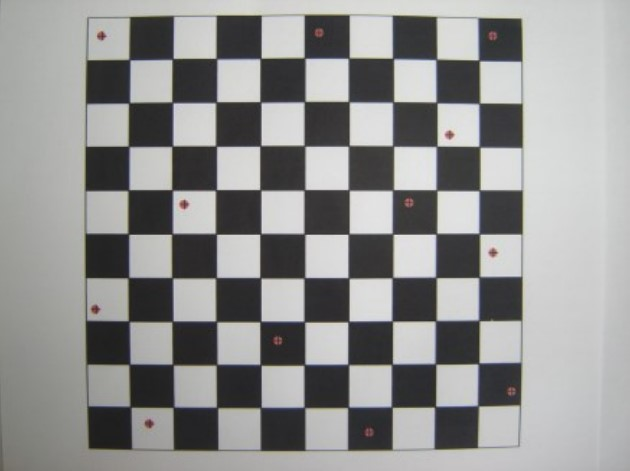
\includegraphics[width=\textwidth]{src/img/mendonca_2013_2d_grid.jpg}
    \caption{2D Referenzraster mit Schachbrettmuster für die Kamerakalibrierung (aus~\cite[Fig. 2]{mendonca_2013})}
    \label{fig:2d_grid}
\end{figure}



\begin{figure}[h]
    \centering
    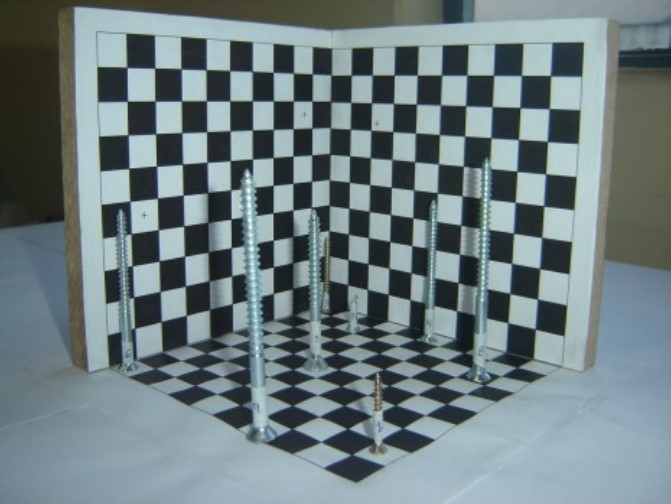
\includegraphics[width=\textwidth]{src/img/mendonca_2013_3d_grid.jpg}
    \caption{3D Referenzraster mit Schachbrettmuster für die Kamerakalibrierung (aus~\cite[Fig. 4]{mendonca_2013})}
    \label{fig:3d_grid}
\end{figure}

